\chapter{Conclusion}
Appendix A provides a calculation to arrive at all critical values of the parameter $t$. These are the values of $t$ where one of the step function that estimates the number of cells in the layers or the number of basis points in the half-shadows has a jump. The approximations of the critical values $t_{r}, r = 1, ..., 43$ of parameter $t$ are:

\begin{align*}
&0.049, \text{\hspace{0.2cm}} 0.075, \text{\hspace{0.2cm}}
0.1, \text{\hspace{0.2cm}} 0.11, \text{\hspace{0.2cm}} 0.19, \text{\hspace{0.2cm}} 0.24, \text{\hspace{0.2cm}} 0.25, \text{\hspace{0.2cm}} 0.25, \text{\hspace{0.2cm}} 0.28, \text{\hspace{0.2cm}} 0.29, \text{\hspace{0.2cm}} 0.29,  \\[6pt]%
&0.33, \text{\hspace{0.2cm}} 0.35, \text{\hspace{0.2cm}} 0.36, \text{\hspace{0.2cm}} 0.37, \text{\hspace{0.2cm}} 0.38, \text{\hspace{0.2cm}} 0.40, \text{\hspace{0.2cm}} 0.43, \text{\hspace{0.2cm}} 0.45, \text{\hspace{0.2cm}} 0.46, \text{\hspace{0.2cm}} 0.47, \text{\hspace{0.2cm}} 0.50.  \\[6pt]
&0.53, \text{\hspace{0.2cm}} 0.54, \text{\hspace{0.2cm}} 0.55, \text{\hspace{0.2cm}} 0.57, \text{\hspace{0.2cm}} 0.60, \text{\hspace{0.2cm}} 0.63, \text{\hspace{0.2cm}} 0.63, \text{\hspace{0.2cm}} 0.64, \text{\hspace{0.2cm}} 0.65, \text{\hspace{0.2cm}} 0.67, \text{\hspace{0.2cm}} 0.71,  \\[6pt]%
&0.71, \text{\hspace{0.2cm}} 0.72, \text{\hspace{0.2cm}} 0.75, \text{\hspace{0.2cm}} 0.75, \text{\hspace{0.2cm}} 0.76, \text{\hspace{0.2cm}} 0.81, \text{\hspace{0.2cm}} 0.89, \text{\hspace{0.2cm}} 0.90, \text{\hspace{0.2cm}} 0.93, \text{\hspace{0.2cm}} 0.95.
\end{align*}

To calculate the sum of all such functions, it suffices to ensure that for an individual value of $t$, at most one of the terms of the sum has a jump. The approximately calculated critical values of the parameter $t$ are limited by the rational numbers $q_{r}, r = 0, ..., 43$:

\begin{align*}
&\frac{1}{40}, \text{\hspace{0.2cm}} \frac{ 1}{16}, \text{\hspace{0.2cm}} \frac{ 1}{11}, \text{\hspace{0.2cm}} \frac{ 2}{19}, \text{\hspace{0.2cm}} \frac{ 1}{6}, \text{\hspace{0.2cm}} \frac{ 1}{5}, \text{\hspace{0.2cm}} \frac{ 5}{21}, \text{\hspace{0.2cm}} \frac{ 26}{103}, \text{\hspace{0.2cm}} \frac{ 3}{11}, \text{\hspace{0.2cm}} \frac{ 2}{7}, \text{\hspace{0.2cm}} \frac{ 5}{17}, \text{\hspace{0.2cm}}\\[6pt]%
&\frac{3}{10}, \text{\hspace{0.2cm}} \frac{ 6}{17}, \text{\hspace{0.2cm}} \frac{ 5}{14}, \text{\hspace{0.2cm}} \frac{ 4}{11}, \text{\hspace{0.2cm}} \frac{ 7}{19}, \text{\hspace{0.2cm}} \frac{ 2}{5}, \text{\hspace{0.2cm}} \frac{ 3}{7}, \text{\hspace{0.2cm}} \frac{ 4}{9}, \text{\hspace{0.2cm}} \frac{ 5}{11}, \text{\hspace{0.2cm}} \frac{ 6}{13}, \text{\hspace{0.2cm}} \frac{ 7}{15}, \text{\hspace{0.2cm}}\\[6pt]%
&\frac{ 8}{15}, \text{\hspace{0.2cm}} \frac{7}{13}, \text{\hspace{0.2cm}} \frac{ 6}{11}, \text{\hspace{0.2cm}} \frac{ 5}{9}, \text{\hspace{0.2cm}} \frac{ 4}{7}, \text{\hspace{0.2cm}} \frac{ 3}{5}, \text{\hspace{0.2cm}} \frac{ 12}{19}, \text{\hspace{0.2cm}} \frac{ 7}{11}, \text{\hspace{0.2cm}} \frac{ 9}{14}, \text{\hspace{0.2cm}} \frac{ 11}{17}, \text{\hspace{0.2cm}} \frac{ 7}{10}, \text{\hspace{0.2cm}} \\[6pt]%
&\frac{ 12}{17}, \text{\hspace{0.2cm}} \frac{5}{7}, \text{\hspace{0.2cm}} \frac{ 8}{11}, \text{\hspace{0.2cm}} \frac{ 77}{103}, \text{\hspace{0.2cm}} \frac{ 16}{21}, \text{\hspace{0.2cm}} \frac{ 4}{5}, \text{\hspace{0.2cm}} \frac{ 5}{6}, \text{\hspace{0.2cm}} \frac{ 17}{19}, \text{\hspace{0.2cm}} \frac{ 9}{10}, \text{\hspace{0.2cm}} \frac{ 13}{14}, \text{\hspace{0.2cm}} \frac{ 20}{21}, \text{\hspace{0.2cm}}
\end{align*}

where each approximation of the critical value $t_{i}$
$$
q_{i-1} < t_{i} < q_{i}
$$
holds. To the sum of step functions that estimate the number of cells in the layers or the number of basis points in the half-shadows, we have added the estimate for the number of points in the central triangle when $h \geq \frac{2}{3}$, see Figure~\ref{fig: all-together-more-than-two-thirds}. The extremum of this function is determined by calculating such a sum for all values of $q_{r}, r = 1,..., 44$. We get the value 101 and our main result, which is summarized by the Theorem~\ref{thm: main}. However, if $h \leq \frac{2}{3}$, we get an estimate of 91. The function obtained in this case is in Figure~\ref{fig: all-together-less-than-two-thirds}.

In Figure~\ref{fig: coverage-mapped} is the division of the frame at one of the critical values $t = \frac{1}{11}$ and $h \geq \frac{2}{3}$, where we get the estimate 101. In Figure~\ref{fig: coverage-final-cells} is the same frame division without using the transformation at the same value of $t$. In Figure~\ref{fig: coverage-final-numbers}, we have marked each region with the maximum number of points it can contain.

\begin{figure}
\centering
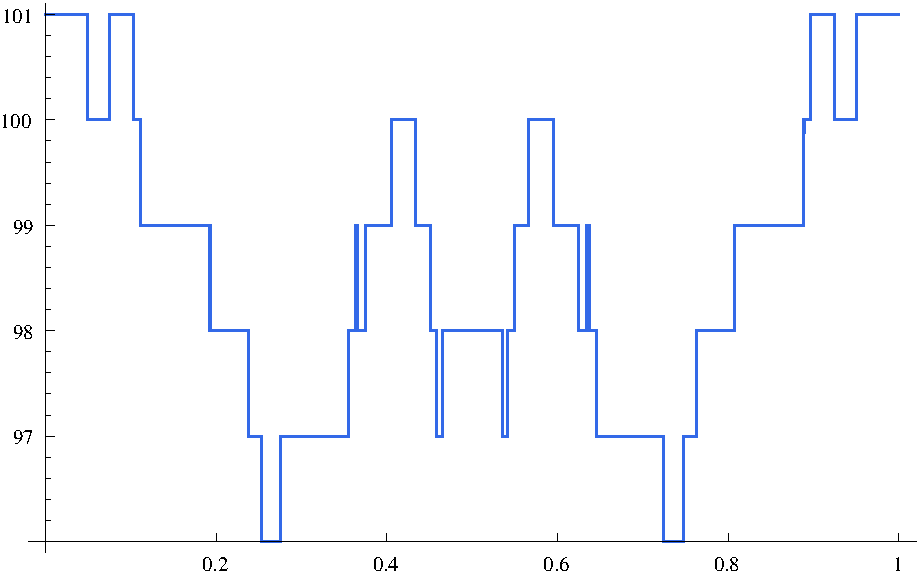
\includegraphics[width=0.8\textwidth]{./figures/all-together-more-than-two-thirds.pdf}
\caption{Plot of the estimate of the number of basis points for $h \geq \frac{2}{3}$.}
\label{fig: all-together-more-than-two-thirds}
\end{figure}

\begin{figure}
\centering
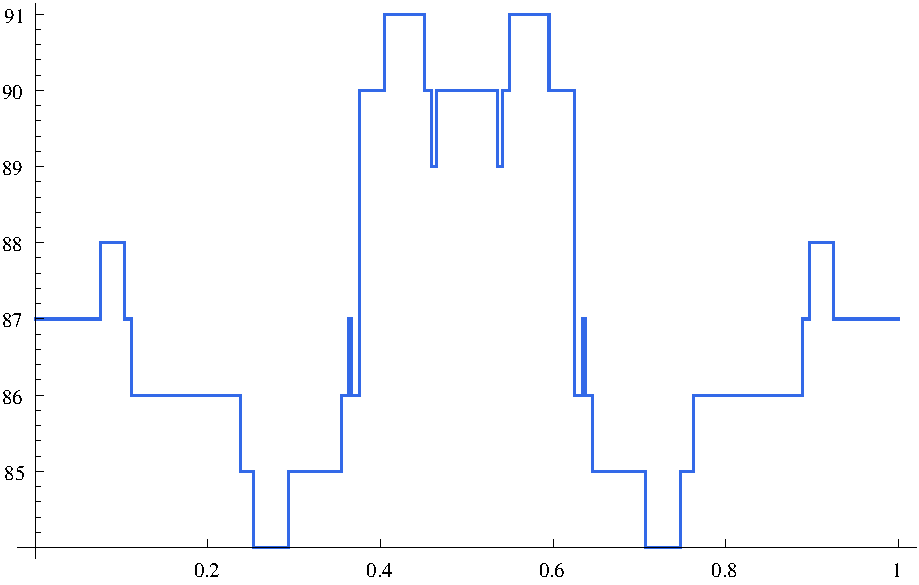
\includegraphics[width=0.8\textwidth]{./figures/all-together-less-than-two-thirds.pdf}
\caption{Plot of the estimate of the number of basis points for $h < \frac{2}{3}$.}
\label{fig: all-together-less-than-two-thirds}
\end{figure}

\begin{figure}
\centering
\begin{tikzpicture}[scale = 4.5, node distance=0.1cm,>=latex, dot/.style={circle,inner sep=1pt,fill,label={#1}, name=#1},
  extended line/.style={shorten >=-#1,shorten <=-#1},
 extended line/.default=1cm]
% S_{ab}
\draw (0,0) -- (-0.166667, -0.288675) -- (0.166667, -0.288675) -- (0.25,0) -- (0,0) -- cycle;
\fill[color-parallelogram,opacity=0.9] (0,0) -- (-0.166667, -0.288675) -- (0.166667, -0.288675) -- (0.25,0) -- (0,0) -- cycle;
% S_{ba}
\draw (1,0) -- (1.16667, -0.288675) -- (0.833333, -0.288675) -- (0.75,0) -- (1,0) -- cycle;
\fill[color-parallelogram,opacity=0.9] (1,0) -- (1.16667, -0.288675) -- (0.833333, -0.288675) -- (0.75,0) -- (1,0) -- cycle;

% S_{bc}
\draw (1,0) -- (1.33333, 0.) -- (1.16667, 0.288675) -- (0.875, 0.216506) -- (1,0) -- cycle;
\fill[color-parallelogram,opacity=0.9] (1,0) -- (1.33333, 0.) -- (1.16667, 0.288675) -- (0.875, 0.216506) -- (1,0) -- cycle;
% S_{cb}
\draw (0.5, 0.866025) -- (0.666667, 1.1547) -- (0.833333, 0.866025) -- (0.625, 0.649519) -- (1,0) -- cycle;
\fill[color-parallelogram,opacity=0.9] (0.5, 0.866025) -- (0.666667, 1.1547) -- (0.833333, 0.866025) -- (0.625, 0.649519) -- (1,0) -- cycle;

% S_{ac}
\draw (0,0) -- (-0.333333, 0.) -- (-0.166667, 0.288675) -- (0.125, 0.216506) -- (0,0) -- cycle;
\fill[color-parallelogram,opacity=0.9] (0,0) -- (-0.333333, 0.) -- (-0.166667, 0.288675) -- (0.125, 0.216506) -- (0,0) -- cycle;
% S_{ca}
\draw (0.5, 0.866025) -- (0.333333, 1.1547) -- (0.166667, 0.866025) -- (0.375, 0.649519) -- (0.5, 0.866025) -- cycle;
\fill[color-parallelogram,opacity=0.9] (0.5, 0.866025) -- (0.333333, 1.1547) -- (0.166667, 0.866025) -- (0.375, 0.649519) -- (0.5, 0.866025) -- cycle;

% color CL
\fill[blue, opacity=0.3] ({-0.2733333333333333}, {-0.5773502691896257}) -- ({-0.00555556},{-0.5773502691896257}) -- ({0.0955556},{-0.28867513459481287})  -- ({-0.13666666666666666},{-0.28867513459481287}) --  ({-0.2733333333333333}, {-0.5773502691896257}) -- cycle;
\fill[blue, opacity=0.3] ({-0.41000000000000003},{-0.8660254037844386})  -- ({-0.137143},{-0.866025}) -- ({-0.0309524},{-0.57735}) -- ({-0.2733333333333333}, {-0.5773502691896257}) -- ({-0.41000000000000003},{-0.8660254037844386}) -- cycle;

% color trapezoids
\fill[grey, opacity=0.3] ({0.3125},{0.2165063509}) -- ({0.2500000000},{0}) -- ({0.7500000000},{0}) -- ({0.6875},{0.2165063509}) -- cycle;
\fill[grey, opacity=0.3] ({0.46875},{0.4871392896}) -- ({0.625},{0.6495190528}) -- ({0.875},{0.2165063509})-- ({0.65625},{0.1623797632}) -- cycle;
\fill[grey, opacity=0.3] ({0.53125},{0.4871392896}) -- ({0.375},{0.6495190528}) -- ({0.125},{0.2165063509}) -- ({0.34375},{0.1623797632}) -- cycle;

\fill[grey, opacity=0.3] ({0.2500000000},{0}) -- ({0.166667},{-0.2886751346}) -- ({0.833333},{-0.2886751346})--({0.7500000000},{0}) -- cycle;

\fill[grey, opacity=0.3] ({0.0955556},{-0.288675}) -- ({-0.00555556},{-0.57735}) -- ({0.954167},{-0.57735})--({0.863333},{-0.288675})-- cycle;
\fill[grey, opacity=0.3] ({-0.0309524},{-0.57735}) -- ({-0.137143},{-0.866025})-- ({0.772},{-0.866025})--({0.726667},{-0.57735}) -- cycle;
\fill[grey, opacity=0.3] ({0.375},{0.6495190528}) -- ({0.329759},{0.696535})-- ({0.0616622},{0.232178})--({0.125},{0.2165063509}) -- cycle;
\fill[grey, opacity=0.3] ({0.875},{0.2165063509}) -- ({1.16667},{0.2886751346}) -- ({0.833333},{0.8660254038})--({0.625},{0.6495190528})-- cycle;
\fill[grey, opacity=0.3] ({1.15018},{0.317225}) -- ({1.43773},{0.396532}) -- ({1.04167},{1.082531755})--({0.833333},{0.8660254038})-- cycle;

% color parallelograms
\node [dot=](a) at (0,0) {};
\node [dot=](b) at (1,0) {};
\node [dot=](c) at ({1/2},{sqrt(3)/2}) {};

%% color deltoids
% deltoid_a
\fill[blue, opacity=0.3] (0,0) -- (0.25,0) -- (0.3, 0.173205) -- (0.125, 0.216506) -- (0,0) -- cycle;
% deltoid_b
\fill[blue, opacity=0.3] (0.75,0) -- (1,0) -- (0.875, 0.216506) -- (0.7, 0.173205) -- (0.75,0) -- cycle;
% deltoid_c
\fill[blue, opacity=0.3] (0.5, 0.866025) -- (0.625, 0.649519) -- (0.5, 0.519615) -- (0.375, 0.649519) -- (0.5, 0.866025) -- cycle;

% color inside
\fill[grey, opacity=0.6] ({0.375}, {sqrt(3)/8}) -- ({0.625}, {sqrt(3)/8}) -- ({0.5}, {sqrt(3)/4}) -- cycle;
\begin{footnotesize}
\node [dot=](a) at (0,0) {};
\node [left = of a] {$a$};
\node [dot=](b) at (1,0) {};
\node [right = of b] {$b$};
\node [dot=](c) at ({1/2},{sqrt(3)/2}) {};
\node [above = of c] {$c$};

\node [dot=](overa) at ({1/2-0.09},{sqrt(3)/2}) {};
\node [above = of overa] {$\abovesym{a}$};
\node [dot=](overb) at ({1/2 + 0.91},{sqrt(3)/2}) {};

\node [dot=](undera) at ({1/2-0.91},{-sqrt(3)/2}) {};
\node [below = of undera] {$\undersym{a}$};
\node [dot=](underb) at ({1/2+0.09},{-sqrt(3)/2}) {};
\node [below = of underb] {$\undersym{b}$};

%[semithick,black]
\draw[ultra thin] (undera) -- (underb) -- (overb) -- (overa) -- (undera) -- cycle;
\draw[thin,dotted] (a) -- (b) -- (c) -- (a) -- cycle;

% big triangle
\draw [thin,dotted] ({-1/2},{-sqrt(3)/2}) -- ({1/2},{sqrt(3)/2}) -- ({3/2},{-sqrt(3)/2}) -- cycle;
% flipud
\draw [thin,dotted] ({-1/2},{sqrt(3)/2}) -- ({1/2},{-sqrt(3)/2}) -- ({3/2},{sqrt(3)/2}) -- cycle;
% draw lower two lines and upper four tilted lines
\draw [thin,dotted]({-1/3},{-sqrt(3)/3}) -- ({4/3},{-sqrt(3)/3});
\draw [thin,dotted]({-1/6},{-sqrt(3)/6}) -- ({7/6},{-sqrt(3)/6});
\draw [thin,dotted]({-1/3},{sqrt(3)/3}) -- ({-1/6},{sqrt(3)/2});
\draw [thin,dotted]({-1/6},{sqrt(3)/6}) -- ({1/6},{sqrt(3)/2});
\draw [thin,dotted]({7/6},{sqrt(3)/6}) -- ({5/6},{sqrt(3)/2});
\draw [thin,dotted]({4/3},{sqrt(3)/3}) -- ({7/6},{sqrt(3)/2});
% halfs frmo 3/4 outwards
\draw [thin,dotted] ({0.5}, {0.2165063509461096}) -- ({1/2},{-sqrt(3)/2});
\draw [ thin,dotted] ({0.5625}, {0.3247595264191645}) -- ({3/2},{sqrt(3)/2});
\draw [ thin,dotted] ({0.4375}, {0.3247595264191645}) -- ({-1/2},{sqrt(3)/2});
% inside deltoids
\draw [ultra thin] ({0.5}, {0.2165063509461096}) -- ({0.5}, {0.28867513459481287});
\draw [ultra thin] ({0.5625}, {0.3247595264191645}) -- ({0.5}, {0.28867513459481287});
\draw [ultra thin] ({0.4375}, {0.3247595264191645}) -- ({0.5}, {0.28867513459481287});

% stubs
\draw[ultra thick] (b) -- ({1 - 0.25*(0.5)}, {0.25*sqrt(3)/2});
\draw[ultra thick] ({1 - 0.75*(0.5)}, {0.75*sqrt(3)/2}) -- (c);
\draw[ultra thick] (a) -- ({0.25*(0.5)}, {0.25*sqrt(3)/2});
\draw[ultra thick] ({0.75*(0.5)}, {0.75*sqrt(3)/2}) -- (c);
\draw[ultra thick] (a) -- ({0.25},0);
\draw[ultra thick] ({0.75}, 0) -- (b);

% symmetrically inside
\draw [ultra thin] ({0.3125},{0.2165063509}) -- ({0.2500000000},{0});
\draw [ultra thin] ({0.375},{0.2165063509}) -- ({0.3333333333},{0});
\draw [ultra thin] ({0.458333},{0.2165063509}) -- ({0.4444444444},{0});
\draw [ultra thin] ({0.541667},{0.2165063509}) -- ({0.5555555556},{0});
\draw [ultra thin] ({0.625},{0.2165063509}) -- ({0.6666666667},{0});
\draw [ultra thin] ({0.6875},{0.2165063509}) -- ({0.7500000000},{0});
\draw [ultra thin] ({0.3125},{0.2165063509}) -- ({0.6875},{0.2165063509});

\draw [ultra thin] ({0.46875},{0.4871392896}) -- ({0.625},{0.6495190528});
\draw [ultra thin] ({0.5},{0.4330127019}) -- ({0.666667},{0.5773502692});
\draw [ultra thin] ({0.541667},{0.3608439182}) -- ({0.722222},{0.4811252243});
\draw [ultra thin] ({0.583333},{0.2886751346}) -- ({0.777778},{0.3849001795});
\draw [ultra thin] ({0.625},{0.2165063509}) -- ({0.833333},{0.2886751346});
\draw [ultra thin] ({0.65625},{0.1623797632}) -- ({0.875},{0.2165063509});
\draw [ultra thin] ({0.46875},{0.4871392896}) -- ({0.65625},{0.1623797632});

\draw [ultra thin] ({0.53125},{0.4871392896}) -- ({0.375},{0.6495190528});
\draw [ultra thin] ({0.5},{0.4330127019}) -- ({0.333333},{0.5773502692});
\draw [ultra thin] ({0.458333},{0.3608439182}) -- ({0.277778},{0.4811252243});
\draw [ultra thin] ({0.416667},{0.2886751346}) -- ({0.222222},{0.3849001795});
\draw [ultra thin] ({0.375},{0.2165063509}) -- ({0.166667},{0.2886751346});
\draw [ultra thin] ({0.34375},{0.1623797632}) -- ({0.125},{0.2165063509});
\draw [ultra thin] ({0.53125},{0.4871392896}) -- ({0.34375},{0.1623797632});

% draw black holes
% BH1
\draw[] ({-0.2733333333333333}, {-0.5773502691896257}) -- ({-0.00555556},{-0.5773502691896257}) -- ({0.0955556},{-0.28867513459481287})  -- ({-0.13666666666666666},{-0.28867513459481287}) --  ({-0.2733333333333333}, {-0.5773502691896257}) -- cycle;
% BH2
\draw[] ({-0.41000000000000003},{-0.8660254037844386})  -- ({-0.137143},{-0.866025}) -- ({-0.0309524},{-0.57735}) -- ({-0.2733333333333333}, {-0.5773502691896257}) -- ({-0.41000000000000003},{-0.8660254037844386}) -- cycle;

% bottom layers
\draw [ultra thin] ({0.2500000000},{0}) -- ({0.166667},{-0.2886751346});
\draw [ultra thin] ({0.3125000000},{0}) -- ({0.25},{-0.2886751346});
\draw [ultra thin] ({0.3906250000},{0}) -- ({0.354167},{-0.2886751346});
\draw [ultra thin] ({0.4882812500},{0}) -- ({0.484375},{-0.2886751346});
\draw [ultra thin] ({0.5117187500},{0}) -- ({0.515625},{-0.2886751346});
\draw [ultra thin] ({0.6093750000},{0}) -- ({0.645833},{-0.2886751346});
\draw [ultra thin] ({0.6875000000},{0}) -- ({0.75},{-0.2886751346});
\draw [ultra thin] ({0.7500000000},{0}) -- ({0.833333},{-0.2886751346});
\draw [ultra thin] ({0.2500000000},{0}) -- ({0.7500000000},{0});

\draw [ultra thin] ({0.0955556},{-0.288675}) -- ({-0.00555556},{-0.57735});
\draw [ultra thin] ({0.148},{-0.288675}) -- ({0.06},{-0.57735});
\draw [ultra thin] ({0.210933},{-0.288675}) -- ({0.138667},{-0.57735});
\draw [ultra thin] ({0.286453},{-0.288675}) -- ({0.233067},{-0.57735});
\draw [ultra thin] ({0.377077},{-0.288675}) -- ({0.346347},{-0.57735});
\draw [ultra thin] ({0.485826},{-0.288675}) -- ({0.482283},{-0.57735});
\draw [ultra thin] ({0.5993},{-0.288675}) -- ({0.624124},{-0.57735});
\draw [ultra thin] ({0.693861},{-0.288675}) -- ({0.742326},{-0.57735});
\draw [ultra thin] ({0.772662},{-0.288675}) -- ({0.840827},{-0.57735});
\draw [ultra thin] ({0.838329},{-0.288675}) -- ({0.922912},{-0.57735});
\draw [ultra thin] ({0.863333},{-0.288675}) -- ({0.954167},{-0.57735});

\draw [ultra thin] ({0.0955556},{-0.288675}) -- ({0.863333},{-0.288675});
\draw [ultra thin] ({-0.00555556},{-0.57735}) -- ({0.954167},{-0.57735}); % lower line

\draw [ultra thin] ({-0.0309524},{-0.57735}) -- ({-0.137143},{-0.866025});
\draw [ultra thin] ({0.0194444},{-0.57735}) -- ({-0.0766667},{-0.866025});
\draw [ultra thin] ({0.0782407},{-0.57735}) -- ({-0.00611111},{-0.866025});
\draw [ultra thin] ({0.146836},{-0.57735}) -- ({0.0762037},{-0.866025});
\draw [ultra thin] ({0.226865},{-0.57735}) -- ({0.172238},{-0.866025});
\draw [ultra thin] ({0.320231},{-0.57735}) -- ({0.284277},{-0.866025});
\draw [ultra thin] ({0.429158},{-0.57735}) -- ({0.41499},{-0.866025});
\draw [ultra thin] ({0.55624},{-0.57735}) -- ({0.567488},{-0.866025});
\draw [ultra thin] ({0.667254},{-0.57735}) -- ({0.700704},{-0.866025});
\draw [ultra thin] ({0.726667},{-0.57735}) -- ({0.772},{-0.866025});
\draw [ultra thin] ({-0.0309524},{-0.57735}) -- ({0.726667},{-0.57735});
\draw [ultra thin] ({-0.137143},{-0.866025}) -- ({0.772},{-0.866025}); % lower line

% upper left part
\draw [ultra thin] ({0.375},{0.6495190528}) -- ({0.329759},{0.696535});
\draw [ultra thin] ({0.336146},{0.582222}) -- ({0.288092},{0.624366});
\draw [ultra thin] ({0.285214},{0.494006}) -- ({0.233474},{0.529765});
\draw [ultra thin] ({0.25},{0.4330127019}) -- ({0.19571},{0.464357});
\draw [ultra thin] ({0.214786},{0.372019}) -- ({0.157947},{0.398948});
\draw [ultra thin] ({0.163854},{0.283804}) -- ({0.103329},{0.304347});
\draw [ultra thin] ({0.125},{0.2165063509}) -- ({0.0616622},{0.232178});
\draw [ultra thin] ({0.375},{0.6495190528}) -- ({0.125},{0.2165063509});
\draw [ultra thin] ({0.329759},{0.696535}) -- ({0.0616622},{0.232178}); % lower line

% upper right part
\draw [ultra thin] ({0.875},{0.2165063509}) -- ({1.16667},{0.2886751346});
\draw [ultra thin] ({0.84375},{0.2706329387}) -- ({1.125},{0.3608439182});
\draw [ultra thin] ({0.804688},{0.3382911734}) -- ({1.07292},{0.4510548978});
\draw [ultra thin] ({0.755859},{0.4228639667}) -- ({1.00781},{0.5638186223});
\draw [ultra thin] ({0.744141},{0.4431614371}) -- ({0.992188},{0.5908819161});
\draw [ultra thin] ({0.695313},{0.5277342304}) -- ({0.927083},{0.7036456406});
\draw [ultra thin] ({0.65625},{0.5953924651}) -- ({0.875},{0.7938566201});
\draw [ultra thin] ({0.625},{0.6495190528}) -- ({0.833333},{0.8660254038});
\draw [ultra thin] ({0.875},{0.2165063509}) -- ({0.625},{0.6495190528});
\draw [ultra thin] ({1.16667},{0.2886751346}) -- ({0.833333},{0.8660254038}); % lower line

\draw [ultra thin] ({1.15018},{0.317225}) -- ({1.43773},{0.396532});
\draw [ultra thin] ({1.11355},{0.380671}) -- ({1.39194},{0.475838});
\draw [ultra thin] ({1.0696},{0.456805}) -- ({1.337},{0.571006});
\draw [ultra thin] ({1.01685},{0.548166}) -- ({1.27106},{0.685207});
\draw [ultra thin] ({0.958486},{0.649255}) -- ({1.19811},{0.811568});
\draw [ultra thin] ({0.909849},{0.733496}) -- ({1.13731},{0.91687});
\draw [ultra thin] ({0.869319},{0.803696}) -- ({1.08665},{1.00462});
\draw [ultra thin] ({0.835544},{0.862197}) -- ({1.04443},{1.07775});
\draw [ultra thin] ({0.833333},{0.8660254038}) -- ({1.04167},{1.082531755});
\draw [ultra thin] ({1.15018},{0.317225}) -- ({0.833333},{0.8660254038});
\draw [ultra thin] ({1.43773},{0.396532}) -- ({1.04167},{1.082531755}); % lower line

\draw [ultra thin] ({1.30037},{0.634451}) -- ({1.49022},{0.727081});
\draw [ultra thin] ({1.23644},{0.745175}) -- ({1.41696},{0.853971});
\draw [ultra thin] ({1.17654},{0.84892}) -- ({1.34832},{0.972862});
\draw [ultra thin] ({1.16667},{0.8660254038}) -- ({1.337},{0.992465});
\draw [ultra thin] ({1.30037},{0.634451}) -- ({1.16667},{0.8660254038});
\draw [ultra thin] ({1.49022},{0.727081}) -- ({1.337},{0.992465}); % lower line

\node [above = of overb] {$\abovesym{b}$};
% color upper 3 trapezoids, so it is grey over b_u
\fill[grey, opacity=0.3] ({1.30037},{0.634451}) -- ({1.49022},{0.727081}) -- ({1.337},{0.992465})-- ({1.16667},{0.8660254038})-- cycle;

% idea from coverage with respect to abd in the upper quadrilateral
%\draw [blue]({-1/3},{sqrt(3)/3}) -- ({4/3},{sqrt(3)/3});

\end{footnotesize}
\end{tikzpicture}
\caption{Transformed frame division at $t=\frac{1}{11}$ in $h \geq \frac{2}{3}$.}
\label{fig: coverage-mapped}
\end{figure}

\begin{figure}[t]%[b]{0.4\textwidth}
\centering
\input{./tikz/coverage-final.subfig}
\caption{Frame division at $t=\frac{1}{11}$ in $h \geq \frac{2}{3}$.}
\label{fig: coverage-final}
\end{figure}

With related methods and a more detailed analysis of estimates in the corner region, we would be able to lower our bound by 1, 2, maybe 3. It also seems that any additional improvement would require more additional pages of text compared to the resulting drop in the estimate. The 101 estimate is a psychological limit. Since it seems that with every improvement we do not produce a large enough drop in estimates, we have almost come to an end with the tools developed. Therefore, we need new methods for something more. We believe that the real number for the order of a complete graph that allows a partial edge drawing is much closer to 16 than 101.

We were also developing the idea of cutting all the layers into finer, denser mesh. This way, we get examples of problems called \textit{maximum independent set problems}. It should work, but we have some reservations. The cell boundaries are selected in a tight manner in each of the layers. When we place a denser mesh over it, we lose on tightness, and maybe the limit increases even more. We don’t have a nice, simple, and effective reason to push points apart instead of allowing them to move. For example, the points in the right triangle may condense toward the point $a$. For a fixed value of the parameter $t$, unoccupied cells could be joined together. However, it is difficult to imagine a unified approach that would work for all possible values of $t$.
